% !TeX root = Protokoll.tex
\subsection{Amplitudenmodulation}
\begin{figure}[h!]
	\centering
	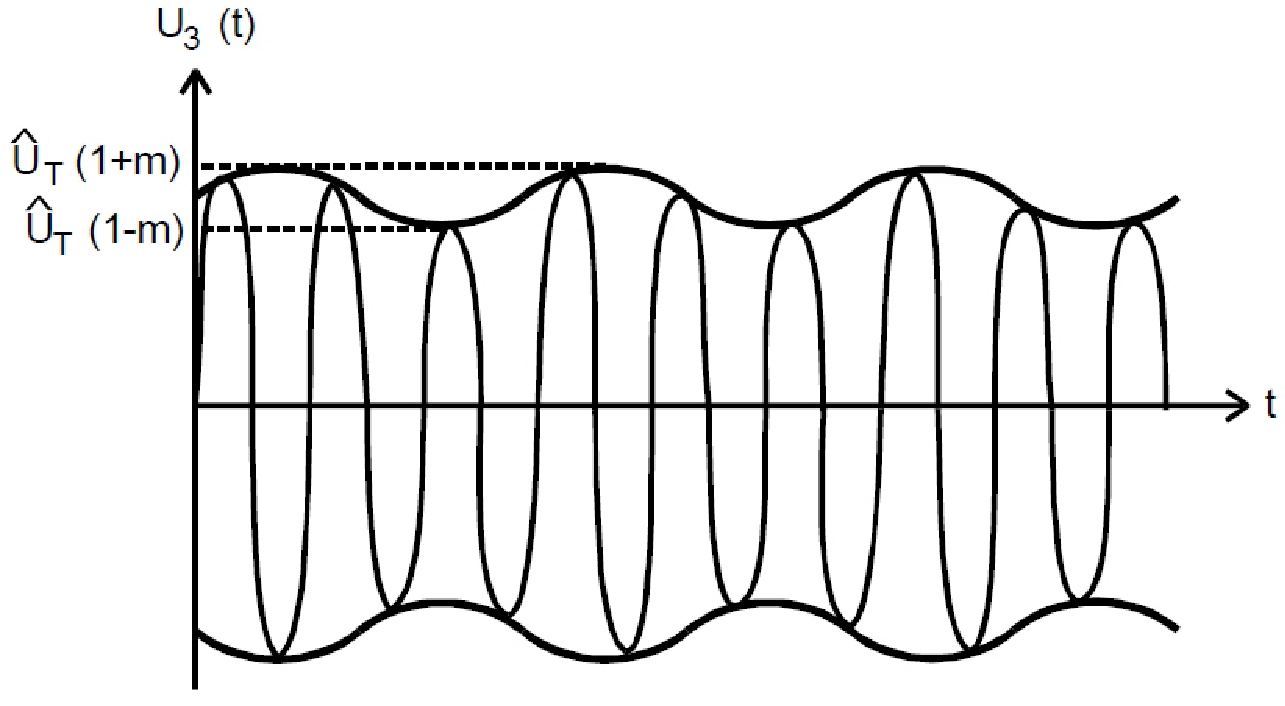
\includegraphics[width = 0.75\textwidth]{../Grafiken/Frequenzbaender.pdf}
	\caption{Beispiel für eine Amplitudenmodulierte Spannung.\cite{V59}\label{fig:modulationsgrad_amplitude}}
\end{figure}
In einer Schaltung ist eine hochfrequente Trägerspannung $U_\text{T}$, die geschrieben werden kann als
\begin{align}
	U_\text{T}(t)=\hat U_\text{T}\cos\omega_\text{T}t.
\end{align}
Dabei ist $\hat U_\text{T}$ die Amplitude und $\omega_\text{T}$ die Kreisfrequenz.
Diese wird mithilfe einer Modulationsspannung $U_\text{M}$ modelliert, diese wird beschrieben durch
\begin{align}
	U_\text{M}(t)=\hat U_\text{M}\cos\omega_\text{M}t,
\end{align}
mit der Amplitude $\hat U_\text{M}$ und der Kreisfrequenz $\omega_\text{M}$.
Die Spannung $U_3$ die aus der Modulation entsteht kann geschrieben werden als
\begin{align}
	U_3(t)=\hat U_\text{T}\left(1+m\cos\omega_\text{M}t\right)\cos \omega_\text{T}t
\end{align}
mit dem Modulationsgrad $m$, der definiert ist als 
\begin{align}
	m = \gamma \hat U_M
\end{align}
mit der Proportionalitätskonstante $\gamma$ mit der Dimension $\frac{1}{\text{V}}$.
Das $m$ liegt zwischen 0 und 1.\\
Die Spannung $U_3$ kann umgeschrieben werden in
\begin{align}
	U_3(t)=\hat U_\text{T} \left[\cos\omega_\text{T}t+\frac{1}{2}m\cos\left(\omega_\text{T}+\omega_\text{M}\right)t+\frac{1}{2}\cos\left(\omega_t-\omega_\text{M}\right)t\right].
\end{align}
Daraus lässt sich das Frequenzspektrum ablesen, dieses ist in \cref{fig:Frequenzspektrum} dargestellt.
Der einfachste Amplitudenmodulator ist die Diode, weil sie eine nicht lineare Kennlinie besitzt.
Durch das anlegen zweier Spannungen, entsteht das Produkt zweier Spannungen. 
\begin{align}
	I(U_\text{T}+U_\text{M})=a_0+a_1(U_\text{T}+U_\text{M})+a_2\left(U_\text{T}^2+U_\text{M} 2\right)+2a_2U_\text{M}U_\text{T}
\end{align}
Allerdings treten in der Reihenentwicklung der Diode auch unerwünschte Terme auf, wie zum Beispiel $U_\text{T}$, $U_\text{M}^2$ und $U_\text{T}^2$.

\begin{figure}
	\centering
	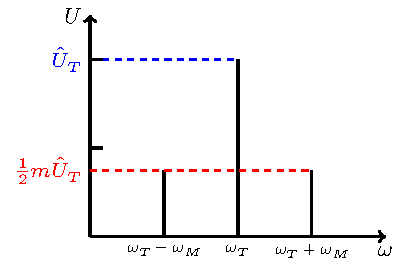
\includegraphics[width =\textwidth/2]{../Grafiken/tikz/tikz-Frequenzspektrum.pdf}
	\caption{Das Frequenzspektrum zu der Amplitudenmodulation.\label{fig:Frequenzspektrum} }
\end{figure}
\newpage
\begin{figure}
	\centering
	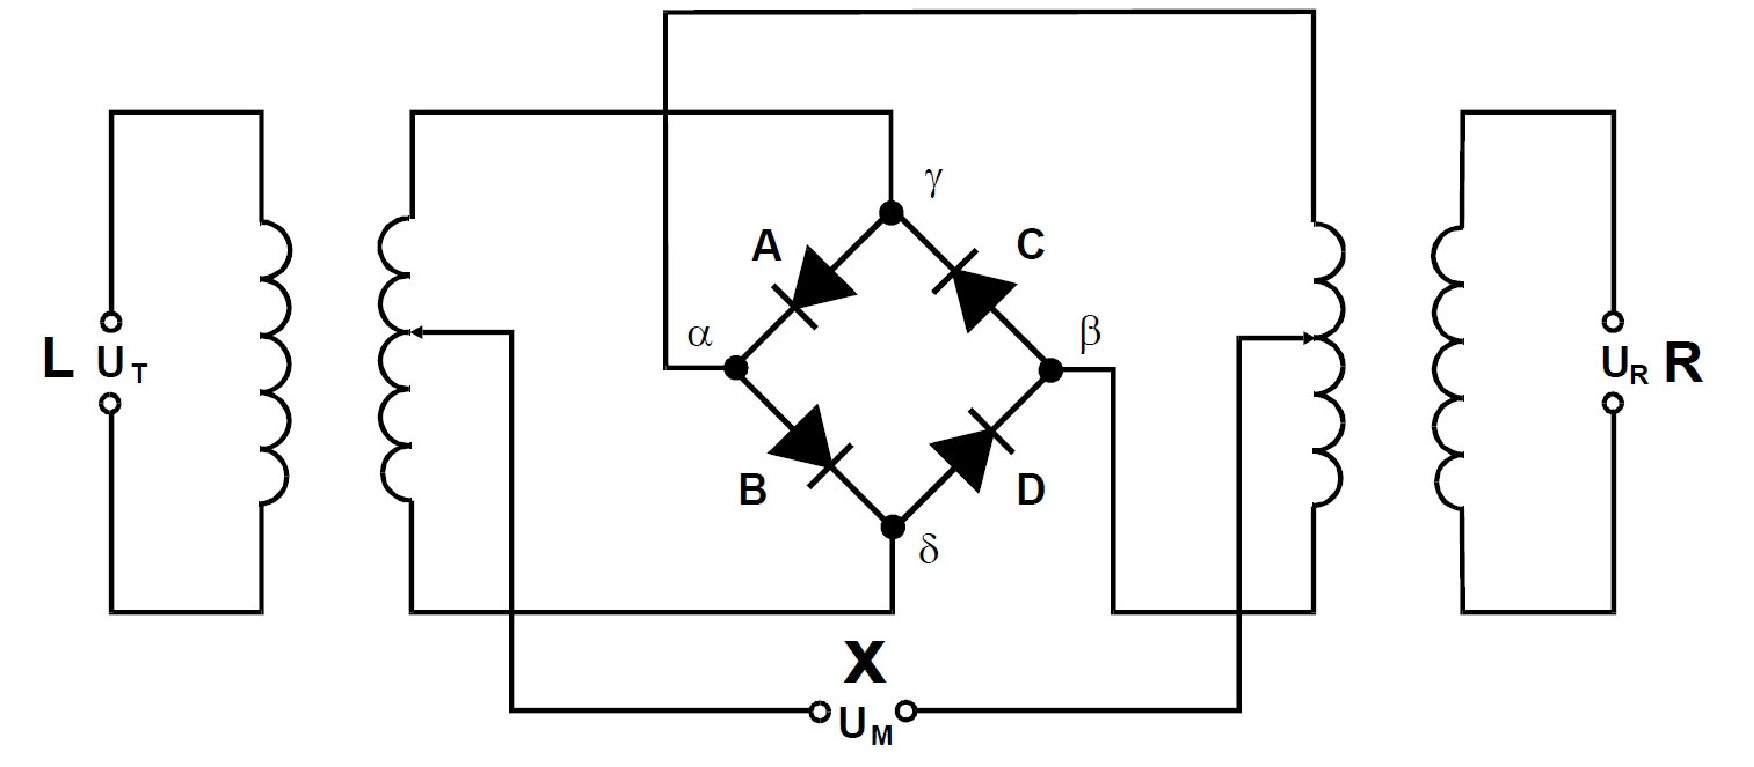
\includegraphics[width = 0.75\textwidth]{../Grafiken/Ringmodulator.pdf}
	\caption{Eine Skizze eines Ringmodulators.\cite{V59}\label{fig:Ringmodulator}}
\end{figure}
Um dies zu umgehen wird ein Ringmodulator verwendet, der besteht aus 4 im Ring angeordneten Dioden, wie in \cref{fig:Ringmodulator} dargestellt.
Am Punkt L liegt die Trägerspannung an und am Punkt X die Modulationsspannung.
Daraus folgt für die modulierte Spannung am Punkt R
\begin{align}
	U_\text{R}(t)=\gamma\cdot \hat U_\text{M}(t) \cdot\hat U_\text{T}(t),
\end{align}
wobei $\gamma$ eine Proportionalitätkonstante ist. Unter Berücksichtigung, dass die Spannung $U_\text{M}$ und $U_\text{T}$ um eine Phase $\phi$ verschieden Schwingen können, folgt
\begin{align}
	U_\text{R}(t)=\Gamma\cdot \frac{\hat U_\text{T}\cdot\hat U_\text{M}}{2}\left[ \left(\cos\left(\omega_\text{T}+\omega_\text{M}\right)t+\phi\right) +\cos\left(\left(\omega_\text{T}-\omega_\text{M}\right)t-\phi\right) \right].
	\label{eq:amplituden_moduliert_ohne_traeger}
\end{align}
Daraus lässt sich erkennen das nur noch die beiden Äußeren Frequenzen des Spektrums auftreten.

\newpage
\subsection{Frequenzmodulation}
\begin{figure}[h!]
	\centering
	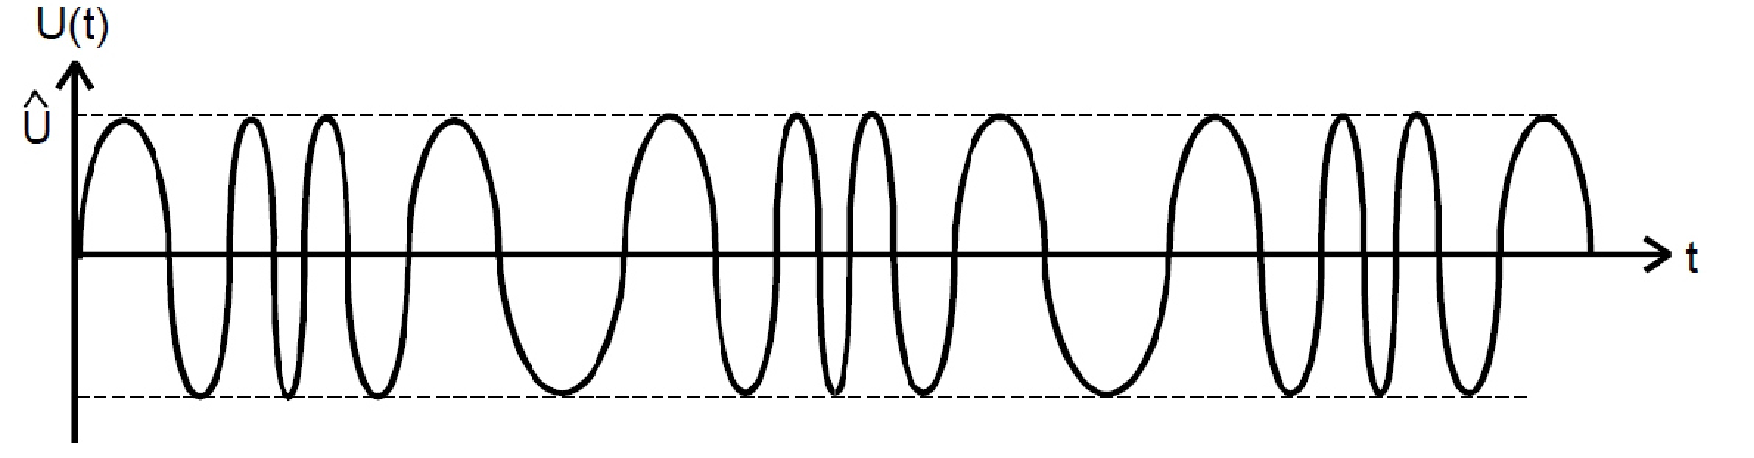
\includegraphics[width = \textwidth]{../Grafiken/Frequenzmodulation.pdf}
	\caption{Darstellung der Änderung einer Frequenzmodulierten Spannung gegen die Zeit.\cite{V59}\label{fig:Frequenzmodulation}}
\end{figure}
Bei der frequenzmodulierten Spannung, ändert sich die Phase beziehungsweise die Frequenz periodisch, wie in \cref{fig:Frequenzmodulation} dargestellt.
Die Spannung einer solcher modulierten Schwingung kann dargestellt werden durch
\begin{align}
	U(t)=\hat U \sin\left(\omega_\text{T}t+m\frac{\omega_\text{T}}{\omega_\text{M}}\cos\omega_\text{M}t\right)
\end{align}
Daraus lässt sich die momentan Frequenz $f$ bestimmen, durch Ableitung des Arguments vom Sinus.
\begin{align}
	f(t)=\frac{\omega_\text{T}}{2\pi}\left(1-m\sin\omega_\text{M}t\right)
\end{align}
Daraus lässt sich der Frequenzhub ablesen als
\begin{align}
	\Delta \omega = m\frac{\omega_\text{T}}{2\pi}
	\label{eq:frequenzhub}
\end{align}
\begin{figure}
	\centering
		\begin{tikzpicture}
			\node [draw=white, anchor=south west] (label) at (0,0) {
				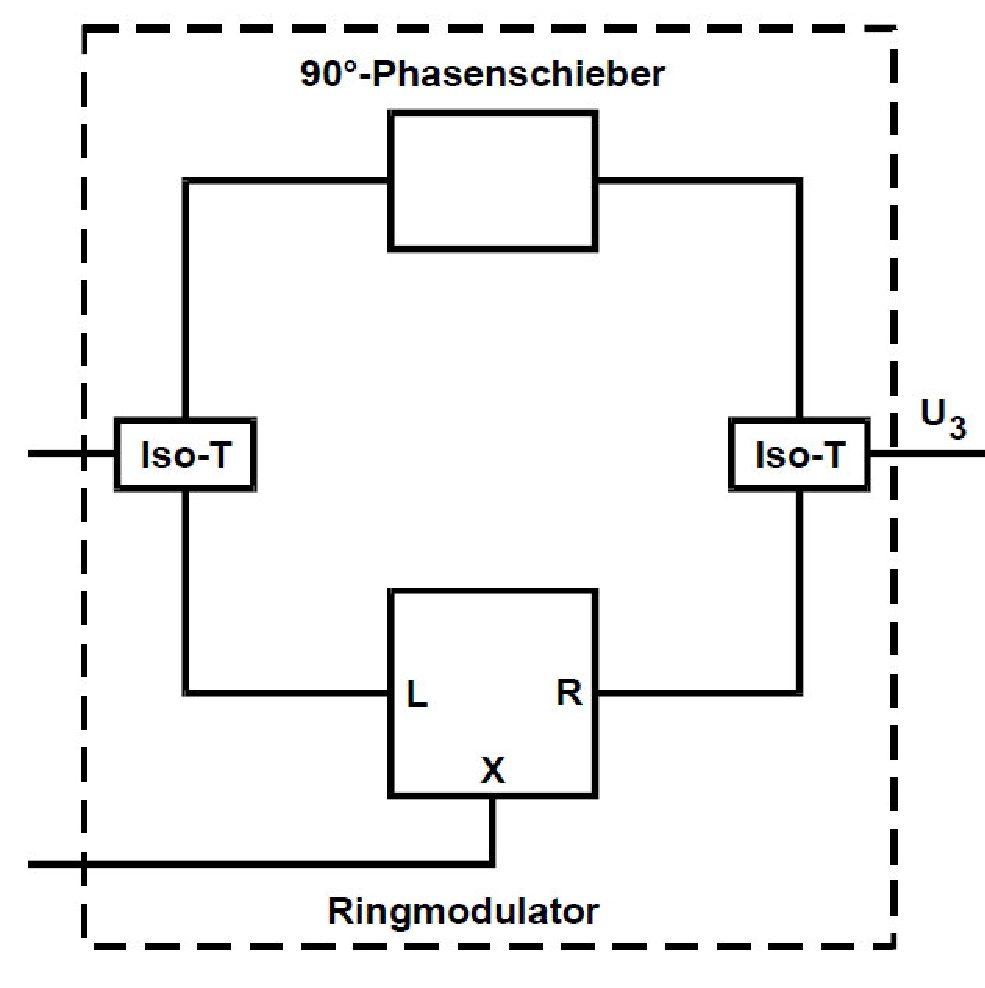
\includegraphics[width=\textwidth/2]{../Grafiken/Schaltung_Frequenzmodulation}};
			\node at (0.9 , 1.4) [left]{$\boldsymbol{U_\text{M}}$};
			\node at (0.9 , 4.75) [left]{$\boldsymbol{U_\text{T}}$};
						
			\fill[white] (7.9,4.92) circle(0.4);
			\node at (8,4.75){$\boldsymbol U_3$};
		\end{tikzpicture}
	\caption{Schaltung für eine Frequenzmodulation.\cite{V59}\label{fig:Schaltung_Frequenzmodlation}}
\end{figure}
Eine Schaltung für eine Frequenzmodulation ist in \cref{fig:Schaltung_Frequenzmodlation} dargestellt.
Dabei wird ein Ringmodulator verwendet, der nur noch Frequenzen $\omega_\text{T}+\omega_\text{M}$ und $\omega_\text{T}-\omega_\text{M}$ zulässt.
Zusätzlich wird ein $90^\circ$-Phasenschifter verwendet, mit dem die phasenverschobene Trägerspannung auf die Spannung der modellierten auf addiert wird.
Daraus entsteht eine frequenzmodulierte Schwingung

\newpage
\subsection{Demodulation von Schwingungen}
Eine Möglichkeit amplitudenmodulierte Schwingungen zu demodulieren ist der Ringmodulator.
Wenn am Eingang R eine modellierte Schwingung mit den Frequenzen $\omega_\text{T}+\omega_\text{M} $ und $\omega_\text{T}-\omega_\text{M}$ anliegt und an Eingang L eine Spannung mit der Kreisfrequenz $\omega_\text{T}$, dann liegt am Ausgang X eine Spannung mit den Frequenzen $\omega_\text{M}$, $2\omega_\text{T}+\omega_\text{M} $ und $2\omega_\text{T}+\omega_\text{M} $ an.
Mithilfe eines Tiefpasses kann die Frequenz $\omega_\text{M}$ heraus gefiltert werde. Diese Methode kann nur angewendet werden, wenn die Frequenz der Trägerspannung zur Verfügung steht.\\
Dieses Problem besteht nicht, wenn mithilfe einer Diode und eines Tiefpasses demoduliert wird.
Allerdings ist aufgrund der Kennlinie der Diode eine Verzerrung der Modulationsspannung zu erwarten.
Dies kann verhindert werden, indem eine Gegentaktschaltung verwendet wird.\\
Die Demudulation einer frequenzmodulierten Schwingung, geschieht mithilfe eines LC-Schwingkreises. Dafür wird die Resonanzfrequenz des Schwingkreises so eingestellt, so dass die Trägerfrequenz $\omega_\text{T}$ auf der Steilen Flanke der Resonanzkurve liegt. Dieses Verfahren macht aus der frequenzmodulierten eine Amplitudenmodulierte Spannung.
\newpage
